\documentclass[journal]{IEEEtran}
\usepackage{cite}
\usepackage{amsmath,amssymb,amsfonts}
\usepackage{algorithmic}
\usepackage{graphicx}
\usepackage{textcomp}
\usepackage{xcolor}
\usepackage{url}
\usepackage{hyperref}
\usepackage{tikz}
\usetikzlibrary{arrows.meta,positioning,calc,decorations.pathreplacing}

\definecolor{cblu}{RGB}{60,110,190}
\definecolor{cgrn}{RGB}{40,150,70}
\definecolor{cred}{RGB}{200,50,50}
\definecolor{corn}{RGB}{210,120,30}
\definecolor{cgry}{RGB}{110,110,110}
\definecolor{cpur}{RGB}{130,60,170}

\begin{document}

\title{Risk Management as a Strategic Bridge: Aligning Cybersecurity Architecture with Business Objectives in Modern Organizations}

\author{Ezekiel Ologunde%
\thanks{E. Ologunde is an independent researcher. Email: ologunde@bu.edu}}

\markboth{}%
{Ologunde: Risk Management as a Strategic Bridge}

\maketitle

\begin{abstract}
Cybersecurity has evolved from a purely technical discipline into a critical business
strategic imperative that directly influences organizational performance, profitability,
and resilience. This paper examines the role of risk management as the essential bridge
connecting technical cybersecurity controls with organizational business objectives.
Through analysis of contemporary cyber incidents, including the 2021 Colonial Pipeline
ransomware attack, and recent empirical research on vulnerability management and
organizational adaptation, we demonstrate that mature risk management practices enable
organizations to allocate resources efficiently, prioritize protection efforts
effectively, and maintain business continuity in an evolving threat landscape. We
identify critical barriers to effective risk management implementation, particularly in
small and medium enterprises (SMEs), where limited security literacy among
decision-makers results in misaligned investments and inadequate protection. Our analysis
reveals that organizations with mature risk management programs demonstrate superior
budget allocation effectiveness and enhanced business resilience. We propose a framework
for integrating risk-based thinking into cybersecurity architecture that balances
protection, usability, and cost while accommodating emerging technologies such as
generative artificial intelligence.
\end{abstract}

\begin{IEEEkeywords}
Risk management, cybersecurity strategy, business alignment, vulnerability management,
small and medium enterprises, cyber resilience, NIST Cybersecurity Framework,
strategic cybersecurity
\end{IEEEkeywords}

\section{Introduction}
\IEEEPARstart{T}{he} transformation of cybersecurity from a technical specialty into a
strategic business imperative represents one of the most significant shifts in
organizational risk management over the past decade. The May 2021 Colonial Pipeline
ransomware attack exemplified this evolution: a single cybersecurity incident halted
fuel distribution across the U.S.\ East Coast, created widespread panic buying, prompted
federal emergency declarations, and resulted in a \$4.4 million ransom
payment~\cite{cisa2021colonial}. Figure~\ref{fig:colonial} illustrates how this single
cyber event cascaded into broad business and societal impacts, demonstrating conclusively
that cyber risk constitutes business risk requiring strategic management at the highest
organizational levels.

\begin{figure}[!t]
\centering
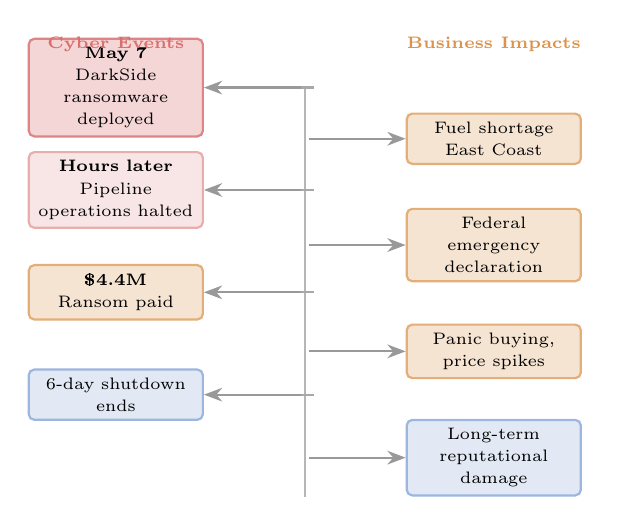
\begin{tikzpicture}[
  font=\fontsize{6.5pt}{8pt}\selectfont,
  >=Stealth,
  ev/.style={rectangle, rounded corners=2pt, draw, thick,
             minimum width=2.2cm, minimum height=0.62cm,
             text centered, text width=2.0cm, inner sep=3pt},
  arr/.style={-{Stealth}, thick, cgry!70}
]
  %% Vertical timeline axis
  \draw[thick, cgry!50] (0,0) -- (0,-5.2);

  %% Events (left side = cyber; right side = business impact)
  \node[ev, fill=cred!20, draw=cred!60] (e1) at (-2.4, 0.00)
    {\textbf{May 7}\\DarkSide ransomware\\ deployed};
  \node[ev, fill=cred!12, draw=cred!40] (e2) at (-2.4,-1.30)
    {\textbf{Hours later}\\Pipeline\\ operations halted};
  \node[ev, fill=corn!20, draw=corn!60] (e3) at ( 2.4,-0.65)
    {Fuel shortage \\ East Coast};
  \node[ev, fill=corn!20, draw=corn!60] (e4) at ( 2.4,-2.00)
    {Federal emergency \\ declaration};
  \node[ev, fill=corn!20, draw=corn!60] (e5) at (-2.4,-2.60)
    {\textbf{\$4.4M}\\Ransom paid};
  \node[ev, fill=corn!20, draw=corn!60] (e6) at ( 2.4,-3.35)
    {Panic buying,\\ price spikes};
  \node[ev, fill=cblu!15, draw=cblu!50] (e7) at (-2.4,-3.90)
    {6-day shutdown\\ ends};
  \node[ev, fill=cblu!15, draw=cblu!50] (e8) at ( 2.4,-4.70)
    {Long-term\\reputational\\damage};

  %% Tick marks on axis
  \foreach \y in {0,-1.30,-2.60,-3.90}{
    \draw[thick, cgry!60] (-0.12,\y) -- (0.12,\y);
  }

  %% Connector arrows: axis → event
  \draw[arr] (-0.05, 0.00) -- (e1.east);
  \draw[arr] (-0.05,-1.30) -- (e2.east);
  \draw[arr] ( 0.05,-0.65) -- (e3.west);
  \draw[arr] ( 0.05,-2.00) -- (e4.west);
  \draw[arr] (-0.05,-2.60) -- (e5.east);
  \draw[arr] ( 0.05,-3.35) -- (e6.west);
  \draw[arr] (-0.05,-3.90) -- (e7.east);
  \draw[arr] ( 0.05,-4.70) -- (e8.west);

  %% Column headers
  \node[font=\fontsize{6pt}{7.5pt}\selectfont\bfseries, text=cred!70]
    at (-2.4, 0.55) {Cyber Events};
  \node[font=\fontsize{6pt}{7.5pt}\selectfont\bfseries, text=corn!80]
    at ( 2.4, 0.55) {Business Impacts};
\end{tikzpicture}
\caption{Colonial Pipeline (May 2021): ransomware compromise cascading from a single
  cyber event into broad operational, economic, and regulatory business impacts.}
\label{fig:colonial}
\end{figure}

Traditional approaches to cybersecurity, characterized by technology-centric
implementations and compliance-driven investments, prove increasingly inadequate.
Organizations face expanding attack surfaces driven by cloud adoption, remote workforce
proliferation, IoT deployment, and digital transformation. Risk management provides the
framework enabling organizations to navigate this landscape strategically, integrating
security into business planning rather than treating it as a cost center~\cite{nist2018framework}.

\subsection{Research Contributions}

This paper: (1)~synthesizes recent empirical research demonstrating the business value of
mature risk management; (2)~analyzes SME-specific challenges including leadership
awareness gaps; (3)~examines emerging risks from generative AI; and (4)~proposes a
practical framework for progressive maturity across organization sizes.

\section{Background and Literature Review}

\subsection{Evolution of Cybersecurity as Business Risk}

Research by the FAIR Institute provides empirical evidence for the business criticality
of risk management. Their 2025 report found that organizations employing quantitative
risk assessment demonstrate 37\% more effective budget allocation and approximately
\$2.3 million lower annual cyber incident costs compared to those with immature
practices~\cite{fairinstitute2025}. Mature programs also correlate with 28\% lower
incident frequency, 41\% shorter mean detection times, and 52\% lower average financial
impact per incident.

\subsection{Risk Management Frameworks}

The NIST Cybersecurity Framework organizes activities into five core functions:
Identify, Protect, Detect, Respond, and Recover~\cite{nist2018framework}. Its tiered
implementation model acknowledges that organizations operate at different maturity levels
and should progress incrementally. ISO~27005 provides complementary guidance on
systematic risk identification, assessment, treatment, and monitoring, emphasizing that
risk management constitutes an ongoing process requiring continuous adaptation as threats,
vulnerabilities, and business contexts evolve~\cite{iso27005}.

\subsection{Quantitative Vulnerability Management}

Shimizu and Hashimoto~\cite{shimizu2025vulnerability} developed a framework incorporating
exploit prediction data to identify vulnerabilities facing the highest probability of
active exploitation. Empirical validation demonstrated 43\% reduction in mean time to
remediation for high-risk vulnerabilities compared to traditional CVSS-based
prioritization. The framework employs machine learning across vulnerability
characteristics, asset criticality, threat intelligence, and organizational context---
illustrating how quantitative approaches enable articulating risk in business terms
suitable for executive decision-making.

\subsection{Organizational Challenges}

Research by Chang et al.~\cite{chang2025mind} found that many SME leaders demonstrate
limited security literacy. Survey data reveals 71\% of SME decision-makers rate their
organization's cyber risk as ``low'' or ``very low,'' despite 58\% of those same
organizations having experienced security incidents in the prior 12 months. Only 34\%
had implemented comprehensive asset inventories---the foundational prerequisite for
effective risk management. Even when leadership recognizes cybersecurity importance,
resource constraints and complexity challenge implementation~\cite{campos2025safeguarding}.

\section{Risk Management as Strategic Bridge}

\subsection{Connecting Technical Controls to Business Objectives}

Risk management functions as the essential bridge connecting technical cybersecurity
implementation with organizational business objectives, as illustrated in
Figure~\ref{fig:bridge}. This bridging role manifests through: \textbf{asset
prioritization} ensuring high-value systems receive proportional protection; \textbf{investment
justification} expressing security needs in business terms (``\$Y million disruption
risk'') rather than technical requirements; and \textbf{balanced decision-making}
navigating trade-offs between protection, usability, cost, and performance.

\begin{figure}[!t]
\centering
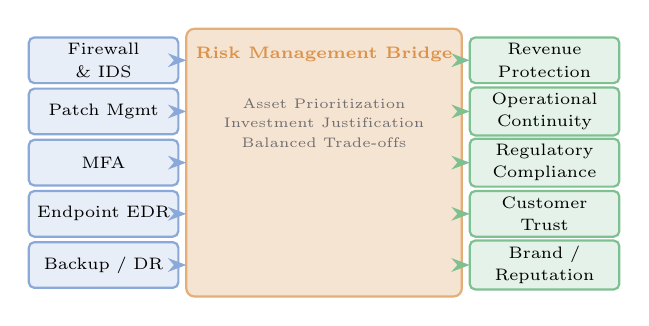
\begin{tikzpicture}[
  font=\fontsize{6.5pt}{8pt}\selectfont,
  >=Stealth,
  lbox/.style={rectangle, rounded corners=2pt, draw=cblu!60, thick,
               fill=cblu!12, minimum width=1.9cm, minimum height=0.58cm,
               text centered, text width=1.7cm, inner sep=2pt},
  rbox/.style={rectangle, rounded corners=2pt, draw=cgrn!60, thick,
               fill=cgrn!12, minimum width=1.9cm, minimum height=0.58cm,
               text centered, text width=1.7cm, inner sep=2pt},
  bridgelabel/.style={font=\fontsize{6pt}{7.5pt}\selectfont\bfseries}
]
  %% Left column — technical controls
  \node[lbox] (t1) at (0,  0.65) {Firewall \& IDS};
  \node[lbox] (t2) at (0,  0.00) {Patch Mgmt};
  \node[lbox] (t3) at (0, -0.65) {MFA};
  \node[lbox] (t4) at (0, -1.30) {Endpoint EDR};
  \node[lbox] (t5) at (0, -1.95) {Backup / DR};

  %% Right column — business objectives
  \node[rbox] (b1) at (5.6,  0.65) {Revenue \\ Protection};
  \node[rbox] (b2) at (5.6,  0.00) {Operational \\ Continuity};
  \node[rbox] (b3) at (5.6, -0.65) {Regulatory \\ Compliance};
  \node[rbox] (b4) at (5.6, -1.30) {Customer \\ Trust};
  \node[rbox] (b5) at (5.6, -1.95) {Brand / \\ Reputation};

  %% Bridge
  \filldraw[fill=corn!20, draw=corn!60, thick, rounded corners=3pt]
    (1.05,-2.35) rectangle (4.55, 1.05);
  \node[bridgelabel, text=corn!80] at (2.80, 0.72)
    {Risk Management Bridge};
  \node[font=\fontsize{5.5pt}{7pt}\selectfont, text=cgry, align=center]
    at (2.80,-0.15) {Asset Prioritization\\Investment Justification\\Balanced Trade-offs};

  %% Arrows left → bridge
  \foreach \y in {0.65,0.00,-0.65,-1.30,-1.95}{
    \draw[-{Stealth}, thick, cblu!60] (0.95,\y) -- (1.05,\y);
  }
  %% Arrows bridge → right
  \foreach \y in {0.65,0.00,-0.65,-1.30,-1.95}{
    \draw[-{Stealth}, thick, cgrn!60] (4.55,\y) -- (4.65,\y);
  }
\end{tikzpicture}
\caption{Risk management as the strategic bridge connecting technical security
  controls (left) to organisational business objectives (right), enabling
  resource prioritisation aligned with mission value.}
\label{fig:bridge}
\end{figure}

\subsection{Empirical Evidence of Business Value}

The 2025 FAIR Institute report surveyed 847 organizations and found quantifiable
differences between mature and immature risk management practices~\cite{fairinstitute2025}.
Organizations with mature programs achieved higher percentages of security budgets directed
toward controls addressing validated high-risk scenarios, reduced expenditure on low-value
compliance controls, and demonstrated stronger alignment between control investments and
organizational risk tolerance. Strategic agility improved as well: organizations with
established risk assessment processes rapidly evaluated security implications of cloud
migrations, acquisitions, and new technology adoptions---allowing security to enable
rather than block business innovation.

\section{Challenges in Small and Medium Enterprises}

\subsection{The Leadership Awareness Gap}

Figure~\ref{fig:awareness_gap} visualizes the perception-reality disconnect among SME
leaders documented by Chang et al.~\cite{chang2025mind}: 71\% rate their own risk as
``low'' while 58\% experienced significant incidents in the prior year; only 34\%
maintain a complete asset inventory despite it being the foundational prerequisite.

\begin{figure}[!t]
\centering
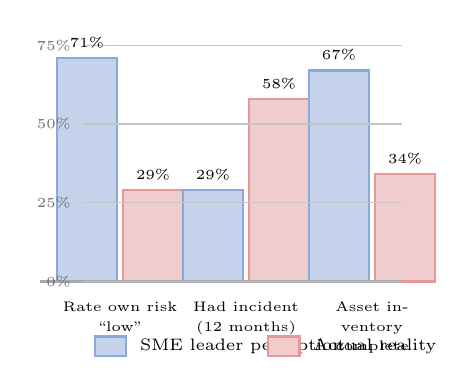
\begin{tikzpicture}[
  font=\fontsize{6.5pt}{8pt}\selectfont,
  >=Stealth
]
  %% ── Bar chart: three metrics, Perception vs Reality ──
  \def\bw{0.38}   %% bar half-width
  \def\gap{1.6}   %% x-gap between groups

  %% Group 1: "Rate risk as Low" (71% perceive; 29% reality inverse)
  \filldraw[fill=cblu!30, draw=cblu!60, thick]
    ({0-\bw},0) rectangle ({0+\bw},2.84);   %% 71%
  \filldraw[fill=cred!25, draw=cred!50, thick]
    ({0+\bw+0.08},0) rectangle ({0+\bw+0.08+2*\bw},1.16); %% 29%

  %% Group 2: "Had incident in prior 12 months" (29% perceive; 58% reality)
  \filldraw[fill=cblu!30, draw=cblu!60, thick]
    ({\gap-\bw},0) rectangle ({\gap+\bw},1.16); %% 29% think at risk
  \filldraw[fill=cred!25, draw=cred!50, thick]
    ({\gap+\bw+0.08},0) rectangle ({\gap+\bw+0.08+2*\bw},2.32); %% 58% had incident

  %% Group 3: "Have asset inventory" (only 34%)
  \filldraw[fill=cblu!30, draw=cblu!60, thick]
    ({2*\gap-\bw},0) rectangle ({2*\gap+\bw},2.68); %% 67% think sufficient
  \filldraw[fill=cred!25, draw=cred!50, thick]
    ({2*\gap+\bw+0.08},0) rectangle ({2*\gap+\bw+0.08+2*\bw},1.36); %% 34% actually have it

  %% X-axis
  \draw[thick, cgry!60] (-0.6,0) -- (4.0,0);

  %% Y-axis labels
  \foreach \y/\pct in {0/0,1/25,2/50,3/75}{
    \draw[cgry!40] (-0.05,\y) -- (4.0,\y);
    \node[anchor=east, font=\fontsize{5.5pt}{7pt}\selectfont, text=cgry]
      at (-0.08,\y) {\pct\%};
  }

  %% Value labels on bars
  \node[above, font=\fontsize{5.5pt}{7pt}\selectfont] at (0,       2.84) {71\%};
  \node[above, font=\fontsize{5.5pt}{7pt}\selectfont] at (0.84,    1.16) {29\%};
  \node[above, font=\fontsize{5.5pt}{7pt}\selectfont] at ({\gap},  1.16) {29\%};
  \node[above, font=\fontsize{5.5pt}{7pt}\selectfont] at ({\gap+0.84}, 2.32) {58\%};
  \node[above, font=\fontsize{5.5pt}{7pt}\selectfont] at ({2*\gap},2.68) {67\%};
  \node[above, font=\fontsize{5.5pt}{7pt}\selectfont] at ({2*\gap+0.84},1.36){34\%};

  %% Group labels below
  \node[below=4pt, text width=1.55cm, align=center,
        font=\fontsize{5.5pt}{7pt}\selectfont] at (0.42,0)
    {Rate own risk\\``low''};
  \node[below=4pt, text width=1.55cm, align=center,
        font=\fontsize{5.5pt}{7pt}\selectfont] at ({1*\gap+0.42},0)
    {Had incident\\(12 months)};
  \node[below=4pt, text width=1.55cm, align=center,
        font=\fontsize{5.5pt}{7pt}\selectfont] at ({2*\gap+0.42},0)
    {Asset inventory\\complete};

  %% Legend
  \filldraw[fill=cblu!30, draw=cblu!60, thick] (0.1,-0.95) rectangle (0.5,-0.70);
  \node[anchor=west, font=\fontsize{6pt}{7.5pt}\selectfont]
    at (0.55,-0.82) {SME leader perception};
  \filldraw[fill=cred!25, draw=cred!50, thick] (2.3,-0.95) rectangle (2.7,-0.70);
  \node[anchor=west, font=\fontsize{6pt}{7.5pt}\selectfont]
    at (2.75,-0.82) {Actual reality};
\end{tikzpicture}
\caption{SME leadership awareness gap (Chang et al.\ 2025): perception versus
  reality across three key metrics. 71\% of SME leaders rate their risk as
  ``low'' yet 58\% experienced a significant incident within 12 months.}
\label{fig:awareness_gap}
\end{figure}

This awareness gap produces misaligned investment priorities---organizations investing in
sophisticated threat intelligence platforms while lacking basic patch management or MFA---
and perpetuates perception of cybersecurity as pure cost center rather than business
resilience investment.

\subsection{Practical Approaches for SMEs}

Campos et al.~\cite{campos2025safeguarding} demonstrate that SMEs achieve substantial
risk reduction through scaled methodologies. A streamlined assessment (typically 20--40
hours) covers: (1)~identifying 5--10 critical assets; (2)~developing 3--5 realistic
threat scenarios; (3)~simplified impact estimation in concrete business terms; (4)~control
gap analysis against CIS Top~5; and (5)~prioritized remediation addressing the highest
risk-exposure gaps first. Even basic quantification---comparing \$50,000 in control costs
against \$500,000 expected annual loss reduced to \$100,000---demonstrates compelling ROI
to business leaders. Managed security service providers offer cost-effective access to
capabilities beyond internal capacity.

\section{Emerging Risk Management Challenges}

\subsection{Generative AI}

Nott~\cite{nott2025organizational} identifies both opportunities and risks from generative
AI in cybersecurity. AI systems can analyze security telemetry at scale, reducing analyst
workload and improving mean time to detect. However, AI integration introduces model
poisoning and adversarial attacks; data leakage through AI responses; AI-enhanced
adversary capabilities for phishing and reconnaissance; and supply chain risks from
third-party AI service dependencies. Effective governance requires approved use case
definitions, human oversight requirements for AI-generated security decisions, and
continuous monitoring of AI system accuracy.

\subsection{Cloud and Third-Party Risk}

Cloud adoption transforms risk management through shared responsibility models where
security obligations distribute between providers and customers. Multi-cloud and hybrid
architectures multiply complexity. Supply chain risks---exemplified by SolarWinds---
demand extending assessment and monitoring to vendor ecosystems, with contractual
right-to-audit provisions and contingency plans for vendor security incidents.

\section{Proposed Framework for Risk-Based Alignment}

\subsection{Framework Components}

The framework comprises five components: (1)~\textbf{Business Context Foundation}
articulating mission, critical assets, stakeholder dependencies, and regulatory
obligations; (2)~\textbf{Risk Assessment} identifying threats, estimating likelihood and
impact, and prioritizing risks requiring treatment; (3)~\textbf{Risk Treatment and Control
Selection} applying the four strategies shown in Figure~\ref{fig:risk_treatment};
(4)~\textbf{Implementation and Operation} with roadmap development, change management,
and operational monitoring; and (5)~\textbf{Continuous Improvement} through metrics,
periodic reassessment, and incident learning.

\begin{figure}[!t]
\centering
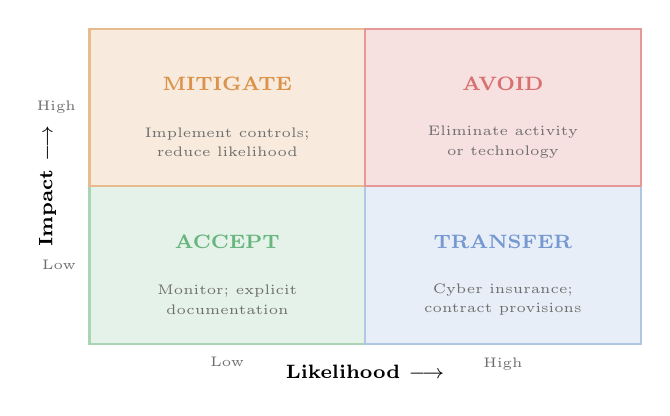
\begin{tikzpicture}[
  font=\fontsize{6.5pt}{8pt}\selectfont,
  >=Stealth
]
  %% Quadrant boxes (2×2 at 3.5cm × 2.0cm each)
  \def\qw{3.5}  \def\qh{2.0}

  %% Low-likelihood / Low-impact → Accept
  \filldraw[fill=cgrn!12, draw=cgrn!40, thick]
    (0,0) rectangle (\qw,\qh);
  \node[font=\fontsize{7.5pt}{9.5pt}\selectfont\bfseries, text=cgrn!70]
    at ({\qw/2},{\qh*0.65}) {ACCEPT};
  \node[font=\fontsize{5.5pt}{7pt}\selectfont, text=cgry, align=center]
    at ({\qw/2},{\qh*0.28}) {Monitor; explicit\\documentation};

  %% High-likelihood / Low-impact → Transfer
  \filldraw[fill=cblu!12, draw=cblu!40, thick]
    (\qw,0) rectangle ({2*\qw},\qh);
  \node[font=\fontsize{7.5pt}{9.5pt}\selectfont\bfseries, text=cblu!70]
    at ({1.5*\qw},{\qh*0.65}) {TRANSFER};
  \node[font=\fontsize{5.5pt}{7pt}\selectfont, text=cgry, align=center]
    at ({1.5*\qw},{\qh*0.28}) {Cyber insurance;\\ contract provisions};

  %% Low-likelihood / High-impact → Mitigate
  \filldraw[fill=corn!15, draw=corn!50, thick]
    (0,\qh) rectangle (\qw,{2*\qh});
  \node[font=\fontsize{7.5pt}{9.5pt}\selectfont\bfseries, text=corn!80]
    at ({\qw/2},{1.65*\qh}) {MITIGATE};
  \node[font=\fontsize{5.5pt}{7pt}\selectfont, text=cgry, align=center]
    at ({\qw/2},{1.28*\qh}) {Implement controls;\\ reduce likelihood};

  %% High-likelihood / High-impact → Avoid
  \filldraw[fill=cred!15, draw=cred!50, thick]
    (\qw,\qh) rectangle ({2*\qw},{2*\qh});
  \node[font=\fontsize{7.5pt}{9.5pt}\selectfont\bfseries, text=cred!70]
    at ({1.5*\qw},{1.65*\qh}) {AVOID};
  \node[font=\fontsize{5.5pt}{7pt}\selectfont, text=cgry, align=center]
    at ({1.5*\qw},{1.28*\qh}) {Eliminate activity\\ or technology};

  %% Axes labels
  \node[rotate=90, anchor=south, font=\fontsize{7pt}{9pt}\selectfont\bfseries]
    at (-0.3,\qh) {Impact $\longrightarrow$};
  \node[anchor=north, font=\fontsize{7pt}{9pt}\selectfont\bfseries]
    at (\qw,-0.15) {Likelihood $\longrightarrow$};

  %% Low/High tick labels
  \node[anchor=east, font=\fontsize{5.5pt}{7pt}\selectfont, text=cgry]
    at (-0.05,{\qh/2}) {Low};
  \node[anchor=east, font=\fontsize{5.5pt}{7pt}\selectfont, text=cgry]
    at (-0.05,{1.5*\qh}) {High};
  \node[anchor=north, font=\fontsize{5.5pt}{7pt}\selectfont, text=cgry]
    at ({\qw/2},-0.05) {Low};
  \node[anchor=north, font=\fontsize{5.5pt}{7pt}\selectfont, text=cgry]
    at ({1.5*\qw},-0.05) {High};
\end{tikzpicture}
\caption{Risk treatment matrix: four strategies mapped to likelihood-impact
  quadrants. High-likelihood/high-impact risks require avoidance; high-impact
  low-likelihood risks warrant mitigation; low-impact risks are transferred or
  accepted based on likelihood.}
\label{fig:risk_treatment}
\end{figure}

\subsection{Maturity Progression}

Figure~\ref{fig:maturity} illustrates the four-level maturity progression, recognizing
that organizations must establish foundations before attempting advanced capabilities.

\begin{figure}[!t]
\centering
\resizebox{\columnwidth}{!}{%
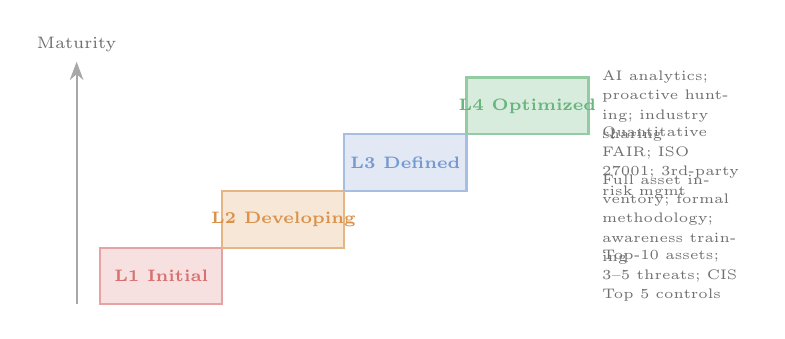
\begin{tikzpicture}[
  font=\fontsize{6.5pt}{8pt}\selectfont,
  >=Stealth
]
  %% Staircase: steps wrapped in resizebox, 0.7cm tall, offset by (1.8, 0.7)
  \def\sw{1.55} \def\sh{0.72}

  \filldraw[fill=cred!15, draw=cred!45, thick]
    (0,0) rectangle (\sw,\sh);
  \filldraw[fill=corn!18, draw=corn!55, thick]
    (\sw,\sh) rectangle ({2*\sw},{2*\sh});
  \filldraw[fill=cblu!15, draw=cblu!45, thick]
    ({2*\sw},{2*\sh}) rectangle ({3*\sw},{3*\sh});
  \filldraw[fill=cgrn!18, draw=cgrn!50, thick]
    ({3*\sw},{3*\sh}) rectangle ({4*\sw},{4*\sh});

  %% Level labels inside steps
  \node[font=\fontsize{6pt}{7.5pt}\selectfont\bfseries, text=cred!70]
    at ({\sw/2},{\sh/2}) {L1 Initial};
  \node[font=\fontsize{6pt}{7.5pt}\selectfont\bfseries, text=corn!80]
    at ({1.5*\sw},{1.5*\sh}) {L2 Developing};
  \node[font=\fontsize{6pt}{7.5pt}\selectfont\bfseries, text=cblu!70]
    at ({2.5*\sw},{2.5*\sh}) {L3 Defined};
  \node[font=\fontsize{6pt}{7.5pt}\selectfont\bfseries, text=cgrn!70]
    at ({3.5*\sw},{3.5*\sh}) {L4 Optimized};

  %% Annotations on right side of each step
  \node[anchor=west, text width=1.85cm,
        font=\fontsize{5.5pt}{7pt}\selectfont, text=cgry]
    at ({4*\sw+0.05},{3.5*\sh})
    {AI analytics; proactive hunting; industry sharing};
  \node[anchor=west, text width=1.85cm,
        font=\fontsize{5.5pt}{7pt}\selectfont, text=cgry]
    at ({4*\sw+0.05},{2.5*\sh})
    {Quantitative FAIR; ISO 27001; 3rd-party risk mgmt};
  \node[anchor=west, text width=1.85cm,
        font=\fontsize{5.5pt}{7pt}\selectfont, text=cgry]
    at ({4*\sw+0.05},{1.5*\sh})
    {Full asset inventory; formal methodology; awareness training};
  \node[anchor=west, text width=1.85cm,
        font=\fontsize{5.5pt}{7pt}\selectfont, text=cgry]
    at ({4*\sw+0.05},{0.5*\sh})
    {Top-10 assets; 3--5 threats; CIS Top 5 controls};

  %% Up arrow on left edge
  \draw[-{Stealth}, thick, cgry!60] (-0.3,0) -- (-0.3,{4*\sh+0.2})
    node[above, font=\fontsize{6pt}{7.5pt}\selectfont, text=cgry]
    {Maturity};
\end{tikzpicture}
}% resizebox
\caption{Risk management maturity progression: four levels from initial
  ad-hoc practices to fully optimised continuous risk analytics, each with
  representative capabilities and controls.}
\label{fig:maturity}
\end{figure}

\textbf{Level~1 (Initial)}: Top 10 critical assets, 3--5 threat scenarios, CIS Top~5
controls, basic incident response. \textbf{Level~2 (Developing)}: Comprehensive asset
inventory, sector-specific threat coverage, CIS Top~10, formal methodology.
\textbf{Level~3 (Defined)}: Quantitative FAIR assessment, ISO~27001, security metrics
integrated with business KPIs, third-party risk programs. \textbf{Level~4 (Optimized)}:
Continuous risk monitoring, predictive AI analytics, security-by-design in all business
processes, proactive threat hunting.

\section{Implementation Recommendations}

\textbf{SMEs}: Invest in executive cybersecurity education; employ simplified
cost-benefit models comparing control costs against expected incident losses; prioritize
foundational controls (MFA, patch management, backups, email security); leverage MSSPs
for capabilities that cannot be built internally; participate in sector ISACs for
collective threat intelligence.

\textbf{Large Enterprises}: Implement comprehensive quantitative FAIR assessment; embed
cybersecurity risk within enterprise risk management with board oversight; deploy
continuous monitoring and automated risk assessment; establish comprehensive third-party
risk programs with ongoing supplier monitoring.

\textbf{All Organizations}: Develop security metrics connected to business outcomes
(incident costs, downtime minutes, customer impact); establish regular executive
risk reporting cadence using business language; conduct tabletop exercises exploring
realistic incident scenarios; explicitly document trade-off decisions between security,
usability, cost, and performance.

\section{Conclusion}

Cybersecurity risk management represents the strategic bridge enabling organizations of
all sizes to connect technical security implementation with business objectives. The
Colonial Pipeline attack demonstrated conclusively that cyber risk constitutes business
risk. Research by the FAIR Institute, Shimizu and Hashimoto, Chang et al., and Campos
et al.\ provides empirical support for the business value of mature risk management:
37\% more effective budget allocation, 52\% lower per-incident financial impact, and
\$2.3 million lower annual incident costs for organizations with mature programs.

SMEs face distinctive barriers---leadership awareness gaps, resource constraints, and
complexity---but scaled methodologies and managed services enable progressive maturity
advancement. Emerging challenges from generative AI, multi-cloud architectures, and
supply chain interdependence require extending risk management frameworks beyond
traditional boundaries.

Six principles emerge: risk management enables strategic alignment ensuring investments
protect assets proportional to business value; quantification improves decision-making
even at simplified levels; maturity progression is appropriate and should precede
advanced capabilities; balance requires explicit consideration of protection-usability-cost
trade-offs; continuous adaptation is essential as threats and contexts evolve; and
leadership engagement is the single most critical factor regardless of technical
sophistication. Organizations that successfully implement these principles will achieve
dual objectives of robust security posture and sustained business performance.

\bibliographystyle{IEEEtran}
\begin{thebibliography}{10}

\bibitem{cisa2021colonial}
CISA, ``DarkSide Ransomware: Best Practices for Preventing Business Disruption,''
Advisory AA21-131A, July~2021.

\bibitem{nist2018framework}
NIST, ``Framework for Improving Critical Infrastructure Cybersecurity, Version 1.1,''
NIST CSWP 04162018, Apr.~2018.

\bibitem{fairinstitute2025}
FAIR Institute, ``2025 State of Cyber Risk Management Report,'' June~2025.

\bibitem{shimizu2025vulnerability}
N.~Shimizu and M.~Hashimoto, ``Vulnerability Management Chaining: An Integrated
Framework for Efficient Cybersecurity Risk Prioritization,'' \textit{Comput.\ Secur.},
vol.~146, p.~103188, 2025.

\bibitem{chang2025mind}
Y.~Chang et al., ``Mind the Gap: Revealing Security Barriers Through Situational
Awareness of SME Key Decision-Makers,'' arXiv:2506.10025, June~2025.

\bibitem{campos2025safeguarding}
J.~Campos, F.~Oliveira, and L.~Pereira, ``Safeguarding the Future: Forecasting
Cybersecurity and Technology Adoption for SMEs,'' \textit{J.\ Bus.\ Continuity Cyber
Resilience}, 2025.

\bibitem{nott2025organizational}
C.~Nott, ``Organizational Adaptation to Generative AI in Cybersecurity: A Systematic
Review,'' arXiv:2506.12060, May~2025.

\bibitem{iso27005}
ISO, ``ISO/IEC 27005:2022 Information Security, Cybersecurity and Privacy
Protection --- Guidance on Managing Information Security Risks,'' Geneva, 2022.

\bibitem{cis2021}
CIS, ``CIS Critical Security Controls Version 8,'' May~2021.

\end{thebibliography}

\end{document}
